\documentclass{standalone}
\usepackage{pgfplots}
\pgfplotsset{compat=1.17}
\usepgfplotslibrary{groupplots}

\begin{document}

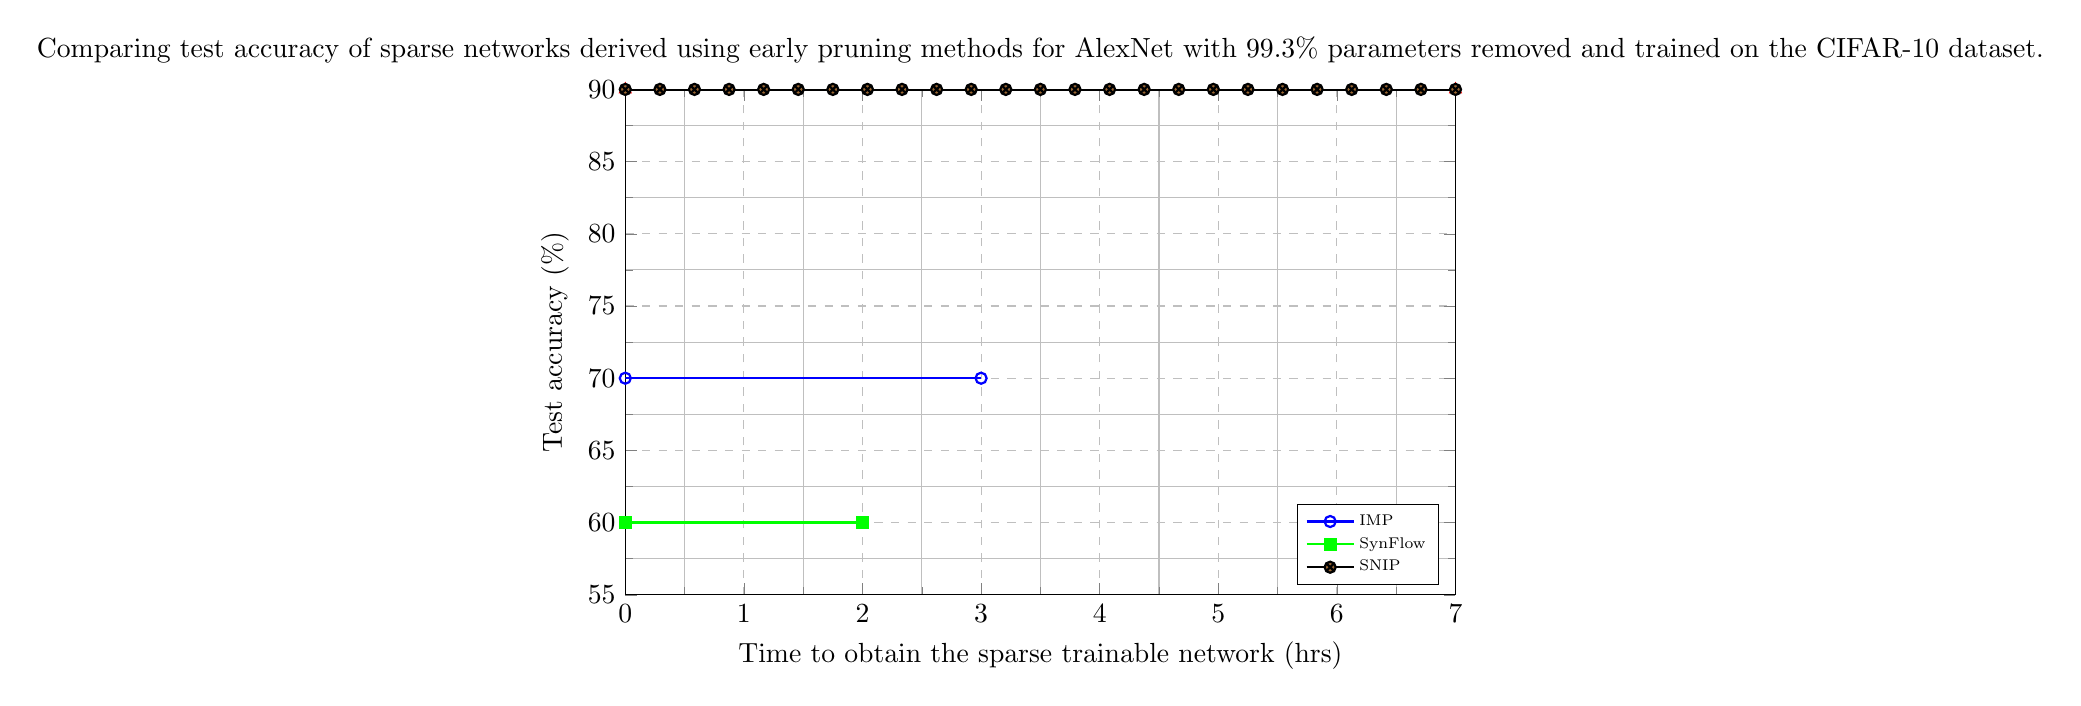
\begin{tikzpicture}
    \begin{axis}[
        width=\textwidth,
        height=8cm,
        title={Comparing test accuracy of sparse networks derived using early pruning methods for AlexNet with 99.3\% parameters removed and trained on the CIFAR-10 dataset.},
        xlabel={Time to obtain the sparse trainable network (hrs)},
        ylabel={Test accuracy (\%)},
        xmin=0, xmax=7,
        ymin=55, ymax=90,
        xtick={0,1,2,3,4,5,6,7},
        ytick={55,60,65,70,75,80,85,90},
        legend pos=south east,
        grid=both,
        major grid style={dashed, gray!50},
        minor tick num=1,
        enlargelimits=false,
        legend cell align={left},
        legend style={at={(0.98,0.02)}, anchor=south east, draw=black, fill=white, nodes={scale=0.8}, font=\scriptsize},
    ]
    
    % IMP (Red Triangle)
    \addplot+[
        mark=triangle*,
        color=red,
        thick,
        mark options={fill=red},
        forget plot
    ] coordinates {
        (0,90)
        (7,90)
    };
    
    % SynFlow (Blue Circle)
    \addplot+[
        mark=o,
        color=blue,
        thick,
        mark options={fill=blue},
    ] coordinates {
        (0,70)
        (3,70)
    };
    
    % SNIP (Green Square)
    \addplot+[
        mark=square*,
        color=green,
        thick,
        mark options={fill=green},
    ] coordinates {
        (0,60)
        (2,60)
    };
    
    % Unpruned Accuracy (Black Line)
    \addplot+[
        color=black,
        thick,
        domain=0:7,
    ] {90};
    
    % Add legends
    \legend{
        IMP,
        SynFlow,
        SNIP,
        Unpruned Accuracy
    }
    \end{axis}
\end{tikzpicture}

\end{document}